\section{Numerical Methods}\label{app:numerical}

%==============================================================================
\subsection{GRMHD Consistency and Convergence}\label{app:resolution_study}

\note{Hector to provide first draft.}

\op{I can put this in}
\note{Brief general discussion of Porth et al. and Olivares et al.}

\note{Comparison of GRMHD output from Illinois/Frankfurt/HAMR}

\note{Comparison of GRMHD output from Illinois at multiple resolutions}

%==============================================================================
\subsection{Radiative Transfer Consistency and Convergence}
\label{app:radtrans}

\bp{Figures here will need to be touched up}

Two studies have been undertaken within the EHT comparing radiative transfer methods used to evaluate models.  The first, \cite{2020ApJ...897..148G}, evaluated the consistency between general relativistic ray-traced radiative transfer (GRRT) codes when tracing geodesics and when integrating the unpolarized radiative transfer equation.  The second, (Prather et al. 2021), evaluates code performance when imaging GRMHD simulation output and when integrating the equations of polarized radiative transfer.

As a  authors and maintainers of several EHT radiative transfer codes participated in a comparison exercise, in which each code produced an image of the same GRMHD snapshot file, designed to realistically simulate an image of the black hole M87* with a total flux of 0.5 Jy.  Figure \ref{fig:radtrans_grmhd_comp} shows tables comparing the total flux of the resulting images, as well as image differences measured by the mean squared error (MSE) between images, defined as

\begin{align}
    \mathrm{MSE}(A, B) &= \frac{\sum_j|A_j-B_j|^2}{\sum_j|A_j|^2}
\end{align}

summed over each image pixel $j$. All images agree to 0.04 Jy (8\%) in flux, and to a mean squared error of 0.0211, recorded by convention as a percentage 2.11\%.  This level of agreement far exceeds the detector uncertainties in the EHT measurements of SgrA* or M87*, rendering the choice of GRRT code irrelevant in producing images for analyses in this paper.

\begin{figure*}
  \centering
  %\note{altex}
  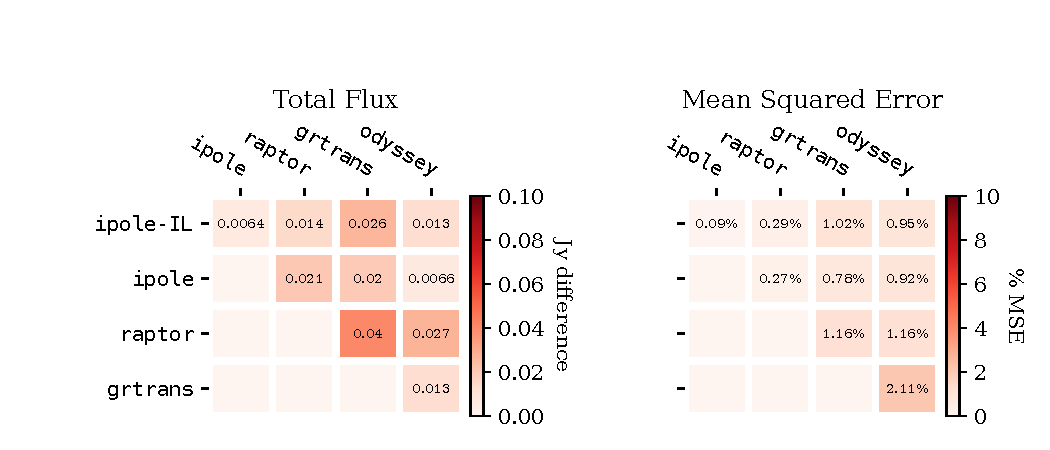
\includegraphics[width=0.9\textwidth]{figures/grmhd_hi_IntegratedUnpolarizeds_plot.pdf}
  \caption{Tables comparing the outputs from several radiative transfer codes used within the EHT for generating images of GRMHD models.  The left table compares total flux between all images (all fluxes were about 0.5 Jy). The right table compares the Mean Squared Error, described in Section \ref{app:radtrans}, which compares image contents.}
  \label{fig:radtrans_grmhd_comp}
\end{figure*}

The image field of view is another potential concern in evaluating models -- the need for efficiency in generating the millions of images used in this analysis was weighed against any emission which might be missed in images with small FOV.  For models which pass size \& other constraints, the FOV is large enough to capture relevant emission, as shown in Figure \ref{fig:radtrans_fov_study}.

\begin{figure}
  \centering
  %\note{altex}
  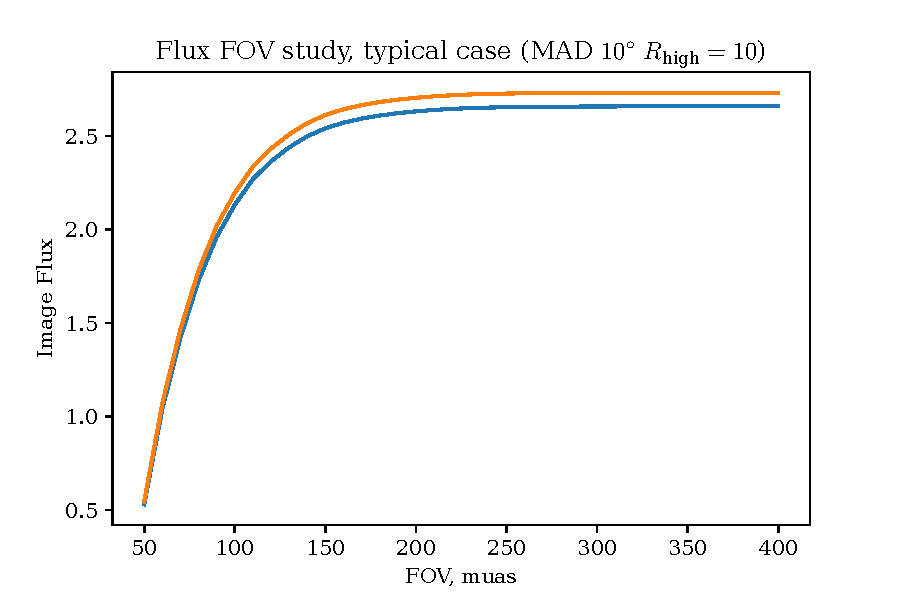
\includegraphics[width=0.45\textwidth]{figures/fov_study.pdf}
  \caption{Flux produced by an image vs the camera field of view.  The nominal FOV of 200 $\mu\mathrm{as}$ is enough to capture 99\% of emission from this model.}
  \label{fig:radtrans_fov_study}
\end{figure}

% Resolution is a much easier sell, we're well converged. Could cite e.g. Gelles+ though that's M87

%==============================================================================
\subsection{Spectral Energy Distribution Consistency and Convergence}

\ckc{CK will do first pass}

\begin{figure*}
    \centering
    %\includegraphics{}
    \note{altex: plot GRRT flux vs SED flux at different wavelengths.  Demonstrates that we have good agreements for 230GHz.  Demonstrate that NIR may require Monty Carlo calculations due to inverse Compton.  Demonstrate some 86GHz images require larger FoV but they are ruled out anyway and would not affect the results.}
    \caption{Comparing GRRT flux from Monte Carlo calculations.  The three columns are 86GHz, 230GHz, and NIR, respectively.  GRRT is only used to spot check x-ray and does not have a corresponding scatter plot.}
    \label{fig:sed_vv}
\end{figure*}

%==============================================================================
\subsection{Cross-Validations}

\ckc{Christian to provide figure}

\begin{figure*}
    \centering
    %\includegraphics{}
    \note{altex: scatter plot between, e.g., Illinois and Frankfurt models for the different measurable.}
    \caption{Comparing model predictions from different modeling pipelines.  ...}
    \label{fig:xv}
\end{figure*}
